\documentclass{article}
\setlength{\parindent}{0 in}
\setlength{\parskip}{0.07 in}

\usepackage[utf8]{inputenc}
\usepackage{graphicx}
\usepackage{setspace}
\usepackage{amsmath,amssymb,amsthm}
\renewcommand{\qedsymbol}{$\blacksquare$}

\usepackage{listings}
\usepackage{xcolor}

\definecolor{dkgreen}{rgb}{0.3,0.5,0.3}
\definecolor{gray}{rgb}{0.5,0.5,0.5}
\definecolor{mauve}{rgb}{0.58,0,0.82}

\lstset{
  language=Java,
  aboveskip=3mm,
  belowskip=3mm,
  showstringspaces=false,
  columns=flexible,
  basicstyle={\ttfamily},
  numbers=left,
  numberstyle=\color{gray},
  keywordstyle=\color{blue},
  commentstyle=\color{dkgreen},
  stringstyle=\color{red!50!brown},
  breaklines=true,
  breakatwhitespace=true,
  tabsize=4
}


\title{Programming Assignment 2:\\ \bigskip
\Large Optimizing Strassen Cut-Off}
\author{Justin Gonzalez}
\date{\today}

\begin{document}

\maketitle
\onehalfspacing
\section{Analytically Solving for $n_0$}
We will begin by solving the recurrence relation for the traditional matrix multiplication algorithm. We know from lecture that when multiplying two $n \times n$ matrices, we need to perform 8 $\frac{n}{2} \times \frac{n}{2}$ matrix multiplications and 4 $\frac{n}{2} \times \frac{n}{2}$ matrix additions for a total $4 (\frac{n}{2})^2$ scalar additions. Therefore our recurrence relation is as follows:
\begin{align*}
    T(n) &= 8 \cdot T(n/2) + 4 \cdot (n/2)^2 \\
    &= 8 \cdot T(n/2) + n^2 \\
    &=8 \cdot (8 \cdot T(n/4) + (n/2)^2) + n^2 \\
    &=8 \cdot (8 \cdot (8 \cdot T(n/8) + \frac{1}{16}n^2) + \frac{1}{4}n^2) + n^2 \\
    &\vdots \\
    &= 8^{\log n - 1} \cdot T(2) + n^2 \sum_{i=0}^{\log n - 2} \frac{8^i}{4^i}
\end{align*}
In our base case of $n=2$, we know that our traditional matrix multiplication algorithm requires 8 scalar multiplications and 4 scalar additions, therefore $T(2)=12$.
\begin{align*}
    T(n) &= \frac{12}{8}n^{\log 8} + n^2 \sum_{i=0}^{\log n - 2} 2^i
\end{align*}
The sum on the right is a geometric series, therefore we can simplify as follows:
\begin{align*}
    T(n) &= \frac{3}{2}n^{3} + n^2 \frac{1-2^{\log n - 1}}{1-2}\\
    &= \frac{3}{2}n^{3} + n^2 \frac{1-\frac{1}{2}n}{-1}\\
    &= \frac{3}{2}n^{3} - n^2 + \frac{1}{2}n^3 \\
    &= 2n^{3} - n^2
\end{align*}
Next we will solve the the recurrence relation for Strassen's algorithm. We know from lecture that when multiplying two $n \times n$ matrices, we need to perform 7 $\frac{n}{2} \times \frac{n}{2}$ matrix multiplications and 18 $\frac{n}{2} \times \frac{n}{2}$ matrix additions and subtractions for a total $18 (\frac{n}{2})^2$ scalar additions and subtractions. Therefore our recurrence relation is as follows:
\begin{align*}
    T(n) &= 7 \cdot T(n/2) + 18 \cdot (n/2)^2 \\
    &= 7 \cdot T(n/2) + \frac{9}{2} \cdot n^2 \\
    &= 7 \cdot (7 \cdot T(n/4) + \frac{9}{2} \cdot (n/2)^2) + \frac{9}{2} \cdot n^2 \\
    &= 7 \cdot (7 \cdot (7 \cdot T(n/8) + \frac{9}{32} \cdot n^2) + \frac{9}{8} \cdot n^2) + \frac{9}{2} \cdot n^2 \\
    &\vdots \\
    &= 7^{\log n - 1} \cdot T(2) + \frac{9}{2}n^2 \sum_{i=0}^{\log n - 2} (\frac{7}{4})^i
\end{align*}
In our base case of $n=2$, we know that our Strassen's algorithm requires 7 scalar multiplications and 18 scalar additions and subtractions, therefore $T(2)=25$.
\begin{align*}
    T(n) &= \frac{25}{7} 7^{\log n} + \frac{9}{2}n^2 \sum_{i=0}^{\log n - 2} (\frac{7}{4})^i
\end{align*}
The sum on the right is a geometric series, therefore we can simplify as follows:
\begin{align*}
    T(n) &= \frac{25}{7} n^{\log 7} + \frac{9}{2}n^2 \frac{1-(\frac{7}{4})^{\log n - 1}}{1-\frac{7}{4}}\\
    &= \frac{25}{7} n^{\log 7} + \frac{9}{2}n^2 \frac{1-\frac{4}{7}(n^{\log \frac{7}{4}})}{-\frac{3}{4}}\\
    &= \frac{25}{7} n^{\log 7} - \frac{36}{6}n^2 (1-\frac{4}{7}n^{\log 7 - 2})\\
    &= \frac{25}{7} n^{\log 7} - 6n^2 + \frac{24}{7}n^{\log 7}\\
    &= 7\cdot n^{\log 7} - 6n^2
\end{align*}
Now we will solve for when the two recurrences are equal. This should give us our rough estimate for $n_0$.
\begin{align*}
    2n^{3} - n^2 &= 7\cdot n^{\log 7} - 6n^2 \\
    0 &= 2n^{3} + 5n^2 - 7\cdot n^{\log 7}
\end{align*}
If we graph the above equation, we see that there is a root near $n=654.031$.
\begin{figure}[htp]
    \centering
    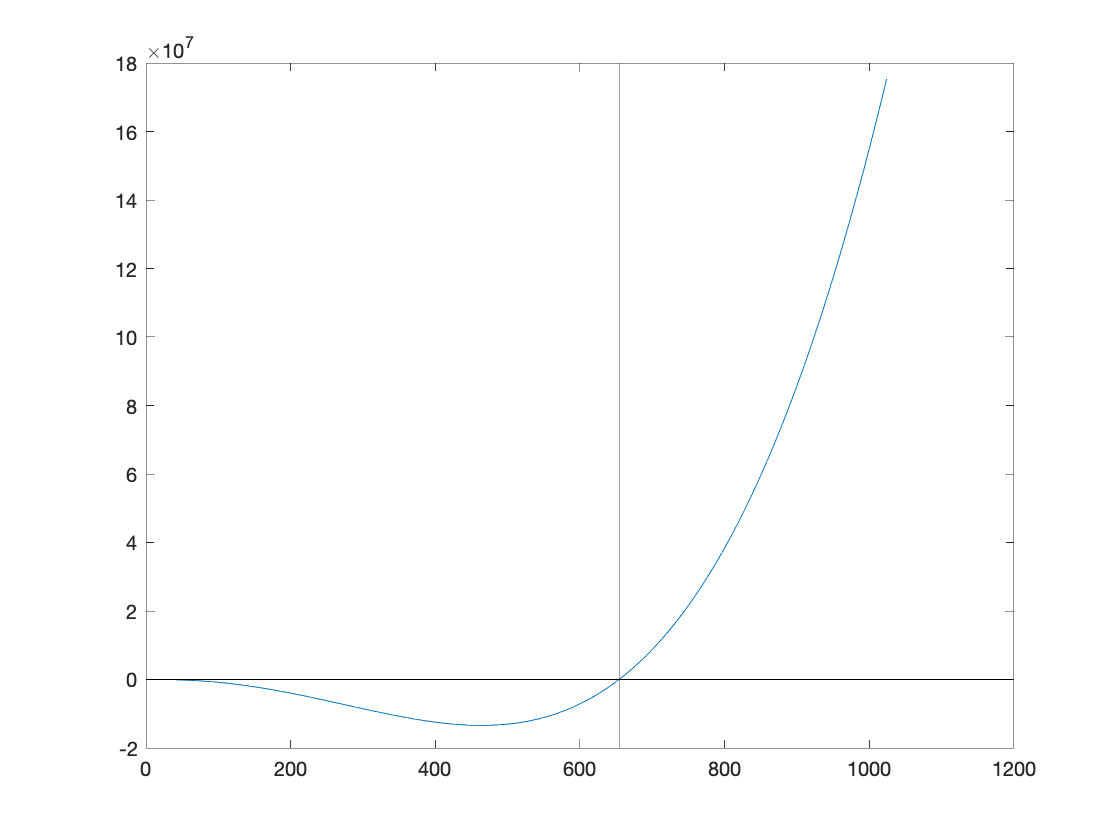
\includegraphics[width=12cm]{root.png}
    \caption{Roots for $n_0$}
    \label{fig:galaxy}
\end{figure}
Therefore, our analytic estimate for $n_0$ is 655. Since our analytic estimate does not account for memory management and treats each operation with uniform cost, we would expect our $n_0$ to be potentially larger than this estimate.

\pagebreak
\section{Empirically Solving for $n_0$}
For my experiment, I set $n = 2n_0$ and incremented $n_0$ until I found an $n_0$ such that running Strassen's algorithm on two random $n \times n$ matrices was faster than the traditional algorithm for matrix multiplication. Using this method, I found that Strassen's algoithm became consistently faster than the traditional algorithm at $n_0 = 46$. The following table displays the running time in seconds for the traditional algorithm and Strassen's algorithm for various $n_0$.

\begin{center}
    \begin{tabular}{ |c|c|c| } 
    \hline
    $n_0$ & Traditional & Strassen\\
    \hline
    35   &   0.000891    &    0.000924\\
    36   &   0.000980    &    0.001026\\
    37   &   0.001102    &    0.001111\\
    38   &   0.001192    &    0.001256\\
    39   &   0.001285    &    0.001264\\
    40   &   0.001489    &    0.001542\\
    41   &   0.001486    &    0.001448\\
    42   &   0.001582    &    0.001627\\
    43   &   0.001685    &    0.001656\\
    44   &   0.001723    &    0.001751\\
    45   &   0.001854    &    0.001855\\
    46   &   0.001987    &    0.001971\\
    47   &   0.002169    &    0.002091\\
    48   &   0.002315    &    0.002211\\
    49   &   0.002567    &    0.002465\\
    50   &   0.002748    &    0.002626\\
    \hline
    
    \end{tabular}
    \end{center}
As we can see, this estimate for $n_0$ is nowhere near our analytic estimate. There are many factors that could be causing these results including my algorithm for traditional matrix multiplication not being fully optimized for memory management. We would expect $n_0$ to be significantly larger than this.
\pagebreak

\section{Triangles in Random Graphs}
\begin{figure}[htp]
    \centering
    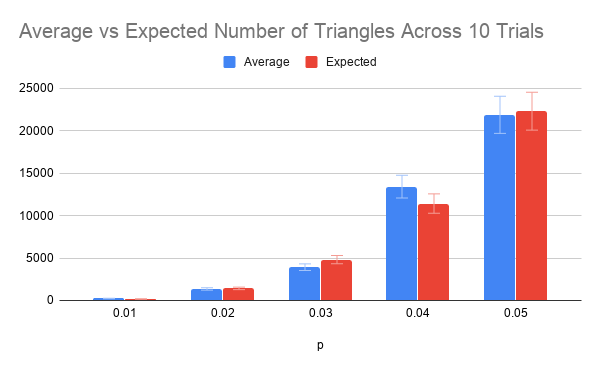
\includegraphics[width=12cm]{avgTriangles.png}
    \caption{Average number of triangles in 10 random graphs for various $p$-values}
    \label{fig:galaxy}
\end{figure}

For this experiment, I generated 10 random undirected graphs and used Strassen's algorithm to find the average number of triangles present for each value of $p$. As we can see from the chart above, my findings appear to be consistent with the expected number of triangles in a graph of size 1024 vertices. Below is a table containing the numerical values of my results.

\begin{center}
    \begin{tabular}{ |c|c|c| } 
    \hline
    $p$ & Average across 10 trials & Expected\\
    \hline
    0.01 & 238.933333  & 178.433024 \\
    0.02 & 1365.333333 & 1427.464192 \\
    0.03 & 3925.333333 & 4817.691648 \\
    0.04 & 13414.4	   & 11419.71354 \\
    0.05 & 21879.46667 & 22304.128\\
    \hline
    
    \end{tabular}
    \end{center}

\end{document}
